\documentclass[12pt]{ctexart}
    %%% Document Settings %%%%
%\usepackage[utf8]{inputenc}

\usepackage[
    twoside,
    top=1in,
    bottom=0.75in,
    inner=0.5in,
    outer=0.5in,
]{geometry}
\pagestyle{myheadings}
\usepackage{minted}
\usepackage[dvipsnames,svgnames]{xcolor}

%%%% Additional Commands to Load %%%%
\usepackage{tcolorbox}
\tcbuselibrary{skins}
\tcbuselibrary{minted}
\usemintedstyle{lovelace}
%\usepackage{minted}
\usepackage{color}
\usepackage{tikz}
\usetikzlibrary{calc}
\usepackage{tabularx,colortbl}
\usepackage{amsfonts,amsmath,amssymb}
\usepackage{titling}
\usepackage{mathrsfs}
\usepackage{calc}
\usepackage{subcaption}

\usepackage{listings}
%\usepackage{newtxtext}
\usepackage[strict]{changepage} 
\usepackage{framed}
\definecolor{formalshade}{rgb}{0.95,0.95,1}
\usepackage{float}

%%%% Commands to Define Homework Boxes %%%%
%%%% Box Definition %%%%
\newtcolorbox{prob}[1]{
% Set box style
    sidebyside,
    sidebyside align=top,
% Dimensions and layout
    width=\textwidth,
    toptitle=2.5pt,
    bottomtitle=2.5pt,
    righthand width=0.20\textwidth,
% Coloring
    colbacktitle=gray!30,
    coltitle=black,
    colback=white,
    colframe=black,
% Title formatting
    title={
        #1 \hfill Grade:\phantom{WWWW}
    },
    fonttitle=\large\bfseries
}

%%%% Environment Definition %%%%
\newenvironment{problem}[1]{
    \begin{prob}{#1}
}
{
    \tcblower
    \centering
    \textit{\scriptsize\bfseries Faculty Comments}
    \vspace{\baselineskip}
    \end{prob}
}

\newenvironment{formal}{%
\def\FrameCommand{%
\hspace{1pt}%
{\color{DarkBlue}\vrule width 2pt}%
{\color{formalshade}\vrule width 4pt}%
\colorbox{formalshade}%
}%
\MakeFramed{\advance\hsize-\width\FrameRestore}%
\noindent\hspace{-4.55pt}% disable indenting first paragraph
\begin{adjustwidth}{}{7pt}%
\vspace{2pt}\vspace{2pt}%
}
{%
\vspace{2pt}\end{adjustwidth}\endMakeFramed%
}

    \title{特殊方程作业5}
    \author{地物2201班\ 杨曜堃}
    \date{\today}
%%% document
\begin{document}

% Format Running Header
    \markboth{\theauthor}{\thetitle}
    \maketitle
    \begin{description}
        \item[问题1] 采用分离变量法求解下列非齐次波动方程。
        $$
        \begin{cases}
            \dfrac{\partial^2 u}{\partial t^2}=\dfrac{\partial^2 u}{\partial x^2}+\sin\pi x,&\quad 0<x<1,\ t>0\\
            u|_{x=0}=0,\ u|_{x=1}=0,&\quad t\geqslant 0\\
            u|_{t=0}=0,\ \dfrac{\partial u}{\partial t}|_{t=0},&\quad 0\leqslant x\leqslant 1
        \end{cases}
        $$
    \end{description}
    % \begin{center}
    %     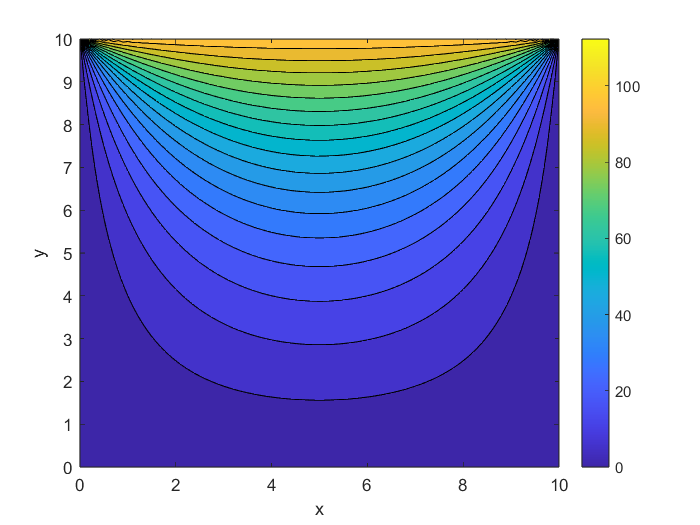
\includegraphics[width=16cm]{fig1.png}
    % \end{center}
    
    \begin{problem}{问题\#1}
        由于非齐次项只是关于$x$的函数,因此可以设
        $$
        u(x,t)=v(x)+w(x,t)
        $$
        代入偏微分方程,可得
        $$
        v''(x)=-\sin\pi x
        $$
        解出
        $$
        v(x)=\dfrac{1}{\pi^2}\sin\pi x+C_1x+C_2
        $$
        代入边界条件
        $$
        v(0)=C_2=0,\ v(1)=C_1+C_2=0,\ C_1=0
        $$
        即
        $$
        v(x)=\dfrac{1}{\pi^2}\sin\pi x
        $$
        而$w(x,t)$是对应齐次定解问题的通解,容易得到
        $$
        w_n(x,t)=\sin n\pi x(C_n\sin n\pi t+D_n\cos n\pi t)
        $$
        代入初始条件
        $$
        D_n\sin n\pi x=-v(x)=-\dfrac{1}{\pi^2}\sin\pi x,\ D_1=-\dfrac{1}{\pi^2}
        $$
        $$
        C_n\sin n\pi x=0,\ C_n=0
        $$
        得到形式解
        $$
        u(x,t)=\dfrac{1}{\pi^2}\sin\pi x(1-\cos\pi t)
        $$
    \end{problem}
\end{document}